\documentclass{beamer}

\usepackage[utf8]{inputenc}
\usepackage[T1]{fontenc}
\usepackage[ngerman]{babel}
\usepackage{amssymb}
\usepackage{amsmath}
\usepackage{amsthm}
\usepackage{graphicx}
\usepackage{caption}

% \usepackage{xcolor}
% \usepackage[Algorithmus]{algorithm}% http://ctan.org/pkg/algorithms
% \usepackage{algpseudocode}% http://ctan.org/pkg/algorithmicx
\usepackage{graphicx}
% \usepackage{wrapfig} % für grafiken mit textumfluss
\usepackage[font=footnotesize]{caption}
\captionsetup{format=plain}
\usepackage{ulem}
\usepackage{hyperref}
% \usepackage[colorlinks, linkcolor = black, citecolor = black, filecolor = black, urlcolor = blue]{hyperref} 


\title{Kontrolltheorie}
\subtitle{Autonome Steuerung einer Mondlandefähre}
\author{Betreuer: Florian Thaler}
\date{08.02.2020}


% getting rid of navigation symbols in the lower right corner
\setbeamertemplate{navigation symbols}{}

\AtBeginSection[]
{
	\begin{frame}
		\frametitle{\normalsize Übersicht}
		\setbeamerfont{block title}{size=\normalsize}
		\normalsize
		\tableofcontents[currentsection]
	\end{frame}
}



\begin{document}


	\begin{frame}[plain]
		\titlepage
	\end{frame}

	\begin{frame}
		\frametitle{Gliederung des Vortrags}
		\tableofcontents
		% fußnote ohne nummerierung
% 		\let\thefootnote\relax\footnote{Durch * gekennzeichnete Abschnitte werden an der Tafel präsentiert.}
	\end{frame}

	\section{Einleitung}
		
		\begin{frame}
 			\frametitle{Kontrolltheorie}
 			\begin{columns}
				\begin{column}{0.48\textwidth}
					\begin{figure}
						
\includegraphics[scale = 0.15]{images/controller.jpg}	
					\end{figure}
				\end{column}
				\begin{column}{0.58\textwidth}
					\begin{itemize}
						\item \textbf{Kontrollsysteme}: Ein mathematisches Modell eines zeitabhängigen Prozesses welches von einem Parameter - einem sogenannten Kontrollparameter - abhängt.
						\item \textbf{Kontrollparameter}: Kann als Steuergröße verstanden werden, welche es erlaubt von außen den Zustand des Systems aktiv zu beeinflussen.
						\item \textbf{Beispiele} finden sich in der Robotik, Finanzwelt ... aber auch in der Luft- und Raumfahrt
					\end{itemize}
				\end{column}
			\end{columns}
		\end{frame}

		\begin{frame}
			\frametitle{Steuerungskonzepte eines dynamischen Systems}
			\begin{columns}
% 				\begin{column}{0.48\textwidth}
% 					\centering
% 					\includegraphics[scale = 0.4]{potential.png}
% 				\end{column}
				\begin{column}{0.58\textwidth}
					\begin{itemize}
						\item \textbf{Regelungstechnik}: Fortlaufendes
							\begin{itemize}
								\item Messen
								\item Vergleichen
								\item Stellen
							\end{itemize}
							um eine Regelgröße auf einen vorgegebenen Sollwert zu bringen. 
						\item \textbf{Optimalsteuerung}: Bestimmung einer Kontrollstrategie zur Minimierung einer gegebenen Kostenfunktion.
					\end{itemize}
				\end{column}
				\begin{column}{0.48\textwidth}
					\begin{figure}
						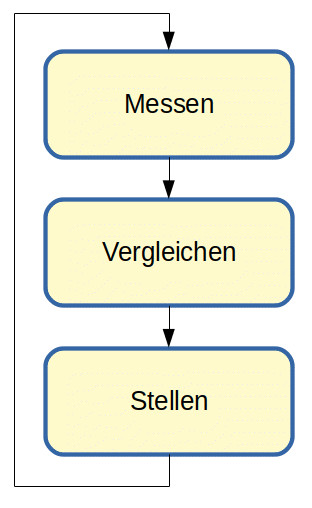
\includegraphics[scale = 0.25]{images/regelkreis.jpg}
						\caption{Regelkreis}
					\end{figure}
				\end{column}
			\end{columns}
		\end{frame}
	\section{Steuerung einer Mondlandefähre}

	\begin{frame}
		\frametitle{Kontrollsystem der Mondlandefähre}
		\begin{columns}
			\begin{column}{0.58\textwidth}
				\begin{itemize}
					\item Formalisierung der \textbf{Zielsetzung}
						\begin{itemize}
							\item Sanfte Landung
							\item Geringer Kraftstoffverbrauch
							\item ...
						\end{itemize}
					\item Aufstellen eines mathematischen Modells und Ableiten der \textbf{Bewegungsgleichungen}
						\begin{align*}
							\dot{x} = f(x, u)
						\end{align*}
					\item Definition der Kontrollparameter $u$ und der Regelgrößen
				\end{itemize}
			\end{column}
			\begin{column}{0.48\textwidth}
				\begin{figure}
					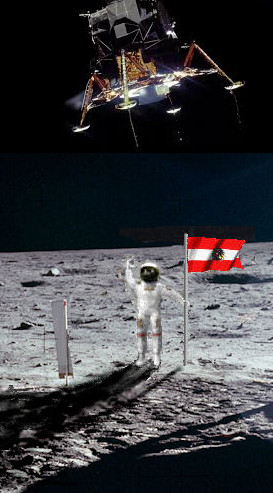
\includegraphics[scale = 0.33]{images/austrianLanding.jpg}	
				\end{figure}
			\end{column}
		\end{columns}
	\end{frame}
		
	\section{Ziele des Projekts}
	
		\begin{frame}
			\frametitle{Ziele des Projekts}
			\begin{columns}
				\begin{column}{0.48\textwidth}
					\begin{figure}
						
\includegraphics[scale = 0.53]{images/projektziele.jpg}	
					\end{figure}
				\end{column}
				\begin{column}{0.58\textwidth}
					\begin{itemize}
						\item Ableitung eines \textbf{mathematischen Modells} zur Beschreibung der Dynamik einer Landefähre.
						\item \textbf{Diskussion verschiedener Kontrollstrategien} zur sanften Landung einer Mondlandefähre.
						\item \textbf{Simulation} des Modells und der Kontrollstrategie am Computer.
						\item Last but not least:
						\pause
						\newline
						\begin{center}
							\large
							\textbf{VIEL FREUDE AN DER MODELLIERUNG}
						\end{center}
					\end{itemize}
				\end{column}

			\end{columns}
		\end{frame}

\end{document}
